\documentclass[preprint,numbers,10pt]{sigplanconf}

\usepackage[utf8]{inputenc}
% the following standard packages may be helpful, but are not required
%\usepackage{longtable}
\usepackage{mathtools}
\usepackage{multicol}
\usepackage{multirow}
\usepackage{booktabs}
\usepackage{courier}
\usepackage[scaled]{helvet}
\usepackage{listings}
\usepackage{enumitem}
\usepackage{mdwlist} % tighter description environment (starred)
\usepackage{gensymb}
\usepackage{hyperref}

\usepackage{graphicx}
\usepackage{softdev}
\usepackage{amsmath}
\usepackage{mdwlist}
\usepackage{pifont}
\usepackage{xspace}

\newcommand{\kalibera}{Kalibera \& Jones\xspace}
\newcommand{\krun}{Krun\xspace}
\newcommand{\hypone}{H1\xspace}
\newcommand{\hyptwo}{H2\xspace}
\newcommand{\binarytrees}{\emph{binary trees}\xspace}
\newcommand{\richards}{\emph{Richards}\xspace}
\newcommand{\spectralnorm}{\emph{spectralnorm}\xspace}
\newcommand{\nbody}{\emph{n-body}\xspace}
\newcommand{\fasta}{\emph{fasta}\xspace}
\newcommand{\fannkuch}{\emph{fannkuch redux}\xspace}
\newcommand{\bencherthree}{Linux1/i7-4709K\xspace}
\newcommand{\bencherfive}{Linux2/i7-4790\xspace}
\newcommand{\benchersix}{OpenBSD/i7-4790\xspace}
\newcommand{\bencherseven}{Linux3/E3-1240v5\xspace}

\newcommand{\flatc}{$\rightarrow$}
\newcommand{\nosteadystate}{$\rightsquigarrow$}
\newcommand{\warmup}{$\uparrow$}
\newcommand{\slowdown}{$\downarrow$}
\newcommand{\inconsistent}{$\rightleftarrows$}

\lstset{
    basicstyle=\tt\scriptsize,
    xleftmargin=2em,
    framexleftmargin=1.5em,
    numberstyle=\scriptsize\tt\color{gray},
    captionpos=b,
    escapeinside={{<!}{!>}},
}

\SDShowCommentTags{default}  %final

\begin{document}

\title{Virtual Machine Warmup Blows Hot and Cold}

\authorinfo{Edd Barrett}{King's College London}{\texttt{http://eddbarrett.co.uk/}}
\authorinfo{Carl Friedrich Bolz}{King's College London}{\texttt{http://cfbolz.de/}}
\authorinfo{Rebecca Killick}{Lancaster University}{\texttt{http://www.lancs.ac.uk/\~{}killick/}}
\authorinfo{Sarah Mount}{King's College London}{\texttt{http://snim2.org/}}
\authorinfo{Laurence Tratt}{King's College London}{\texttt{http://tratt.net/laurie/}}
%\keywords{warmup, benchmarking, virtual machines, programming languages.}

%\authorrunning{E. Barrett, C. F. Bolz, R. Killick, V. Knight, S. Mount, and L. Tratt}

\maketitle

\begin{abstract}
Virtual Machines (VMs) with Just-In-Time (JIT) compilers are traditionally thought
to execute programs in two phases: first the \emph{warmup} phase determines which
parts of a program would most benefit from dynamic compilation; after
compilation has occurred, the program is said to be at \emph{peak performance}.
When measuring the performance of JIT compiling VMs, data collected
during the warmup phase is generally discarded, placing the focus on peak
performance. In this paper we first run a number of small,
deterministic benchmarks on a variety of well known VMs, before introducing
a rigorous statistical model for determining when warmup has occurred.
In our experiment, \laurie{only XXX\%} of the benchmark/VM pairs conform to
the traditional view of warmup, and none of the
VMs we tested consistently warms up.
\end{abstract}

\section{Introduction}
\label{sec:intro}

Many modern languages are implemented as Virtual Machines (VMs) which use a
Just-In-Time (JIT) compiler to translate `hot' parts of a program into efficient
machine code at run-time. Since it takes time to determine which parts of the
program are hot, and then compile them, programs which are JIT compiled are
said to be subject to a \emph{warmup} phase. The traditional view of
JIT compiled VMs is that program execution is slow during the warmup phase, and
fast afterwards, when a steady state of \emph{peak performance} is said to have been reached
(see Figure~\ref{fig:trad} for a simplified view of this).
This traditional view underlies most benchmarking of JIT compiled VMs, which
usually require running benchmarks several times within a single VM process,
discarding any timing data collected before warmup is complete, and
reporting only peak performance figures.

The fundamental aim of this paper is to test the following hypothesis, which captures a constrained
notion of the traditional view of warmup:
\begin{description}
  \item[\hypone] Small, deterministic programs exhibit traditional warmup behaviour.
\end{description}
We present a carefully designed
experiment where a number of simple benchmarks are run on seven
VMs and GCC for a large number of \emph{in-process iterations} and repeated using fresh
\emph{process executions} (i.e.~each process execution runs multiple in-process
iterations). We also introduce the first automated approach to determining
\emph{when} warmup has completed, based on statistical changepoint analysis.

\begin{figure}[t]
\centering
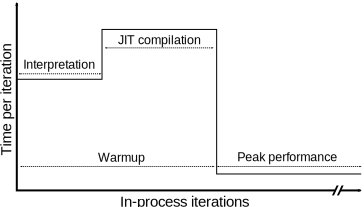
\includegraphics[width=.475\textwidth]{img/picturebook_warmup}
\caption{The traditional view of warmup: a program starts slowly executing in
an interpreter; once hot parts of the program are identified, they are
translated by the JIT compiler to machine code; at this point warmup
is said to have completed, and peak performance reached.}
\label{fig:trad}
\end{figure}

While our results show that some benchmarks on some VMs run as per the traditional
view, many surprising cases exist: some benchmarks slowdown rather than
warmup; some never hit a steady state; and some perform very differently over
different process executions. Of the seven
VMs we looked at, none consistently warms up as per the traditional view.

Our results clearly invalidate Hypothesis H1, showing that the traditional
view of warmup is no longer valid (and, perhaps, that it may not have held in
the past). This is of importance to both VM developers and users:
much prior VM benchmarking is likely to be partly misleading: and it is
likely to have allowed some ineffective, and perhaps some deleterious,
optimisations to be included in production VMs.

\vspace{10pt}

\noindent In order to test Hypothesis H1, we first present a carefully designed
experiment (Section~\ref{sec:methodology}). We then introduce a new
statistical method for automatically determining if/when warmup has occurred,
which allows us to classify benchmarks' warmup style, and present steady-state
in-process iteration times (when possible) based upon the classifications
(Section~\ref{sec:stats}). Since a number of cases fail to warmup in the
traditional fashion, we then run a smaller experiment to understand how JIT
compilation and Garbage Collection (GC) affect warmup
(Section~\ref{sec:deepdive}). As a useful side bonus of our main experiment,
we present data for VM \emph{startup} time: how long it takes until a VM can
start executing any user code (Section~\ref{sec:startup}). Finally, we show that
our statistical method can be applied to well known benchmark suites run in a
conventional manner (Section~\ref{sec:existing}).

The repeatable experiment we designed, as well as the specific results used
in this paper, can be downloaded from:
\vspace{-.5em}
\begin{center}
\url{https://archive.org/download/softdev_warmup_experiment_artefacts/v0.7/}
\end{center}
% should you say where people can get the code to run it themselves?  This sentance just feels like
% it is ``reproducible rersearch'' rather than ``please run it on your own data''.

\section{Background}
\label{sec:warmup}

Figure~\ref{fig:trad} shows the traditional view of warmup.
When a program begins running on a JIT compiled VM, it is typically (slowly)
interpreted; once `hot' (i.e.~frequently executed) loops or methods are
identified, they are dynamically compiled into machine code; and subsequent
executions of those loops or methods use (fast) machine code rather than the
(slow) interpreter. Once machine code generation has completed, the VM is
said to have finished warming up, and the program to be executing
at a steady state of peak performance.\footnote{The traditional view applies equally to VMs
that perform immediate compilation instead of using an interpreter, and to
those VMs which have more than one layer of JIT compilation (later JIT
compilation is used for `very hot' portions of a program, trading slower
compilation time for better machine code generation).}
While the length of the warmup period
is dependent on the program and JIT compiler, all JIT compiling
VMs assume this performance model holds true~\cite{kalibera13rigorous}.

Benchmarking of JIT compiled VMs typically focusses on peak
performance, partly due to an assumption that
warmup is both fast and inconsequential to users.
The methodologies used are typically straightforward: benchmarks are run for a number
of in-process iterations within a single VM process execution.
The first $n$ in-process iterations\footnote{In our experience, often hard-coded
to 5.} are then discarded, on the basis that warmup should have completed in
that period: however, no guarantees can be made that it has completed.

A more sophisticated VM benchmarking methodology
was developed by \kalibera~\cite{kalibera12quantifying,kalibera13rigorous}. The basic idea is
that, for a given VM / benchmark combination, a human must inspect data obtained by
executing a small number of process executions, and determine at which in-process iteration the
benchmark has definitively warmed up. A larger number of VM process executions are then
run, and the previously determined cut-off point applied to each process's
iterations. The \kalibera methodology observes that some benchmarks do not
obviously warm up; and that others follow cyclic patterns post-warmup
(e.g.~in-process iteration $m$ is slow, $m+1$ is fast, for all even values of $m > n$). In
the latter case, the \kalibera methodology requires a consistent in-process iteration in
the cycle (ideally the first post-warmup iteration) be picked for all process
executions, and used for statistical analysis.

Although the \kalibera methodology is the most
sophisticated currently available,
there remain cases where it remains hard to produce satisfying benchmarking
statistics. Crucially, as it relies on human expertise, the methodology does not
provide a repeatable way of determining when warmup has completed. Because of this
``determining when a system has warmed up, or even providing a
rigorous definition of the term, is an open research problem''~\cite{seaton15phd}.


\section{Methodology}
\label{sec:methodology}

To test Hypothesis H1, we designed an experiment which uses a suite of
micro-benchmarks: each is run with 2000 in-process iterations and repeated
using 10 process executions. We have carefully designed our
experiment to be repeatable and to control as many potentially confounding variables as
is practical. In this section we detail: the benchmarks we used and the modifications we
applied; the VMs we benchmarked; the machines we used for benchmarking; and the
\krun system we developed to run benchmarks.


\subsection{The Micro-benchmarks}

The micro-benchmarks we use are as follows: \binarytrees, \spectralnorm, \nbody,
\fasta, and \fannkuch from the Computer Language Benchmarks Game (CLBG)~\cite{clbg}; and
\richards. Readers can be forgiven for initial scepticism about this set of micro-benchmarks.
They are small and widely
used by VM authors as optimisation targets. In general they are more effectively
optimised by VMs than average programs; when used as a proxy for other types
of programs (e.g.~large programs), they tend to overstate the effectiveness of
VM optimisations (see e.g.~\cite{ratanaworabhan09jsmeter}). In our context, this weakness is in fact a strength:
small, deterministic, and widely examined programs are our most
reliable means of testing Hypothesis H1. Put another way, if we were to run arbitrary programs
and find unusual warmup behaviour, a VM author might reasonably counter that
``you have found the one program that exhibits unusual warmup behaviour''.

For each benchmark, we provide versions in C, Java, Javascript, Python, Lua, PHP,
and Ruby. Since most of these
benchmarks have multiple implementations in any given language, we picked
the versions used in~\cite{bolz14impact}, which represented the fastest
performers at the point of that publication. We lightly modified
the benchmarks to integrate with our benchmark runner (see Section~\ref{krun}).
For the avoidance of doubt we did not interfere with any VM's GC (e.g.~we did not
force a collection after each iteration).


\subsubsection{Ensuring Determinism}

User programs that are deliberately non-deterministic programs are unlikely to
warm-up in the traditional fashion.
We therefore wish to guarantee that our benchmarks are,
to the extent controllable by the user, deterministic: that they
take the same path through the Control Flow Graph (CFG)
on all process executions and in-process iterations.\footnote{Note that non-determinism
beyond that controllable by the user (i.e.~non-determinism in low-level parts of
the VM) is part of what we need to test for Hypothesis H1.}

To check whether the benchmarks were deterministic at the user-level, we created
versions with \texttt{print} statements at all possible points of CFG
divergence (e.g.~\texttt{if} statements' true and false branches).
These versions are available in our experimental suite. We first ran the modified
benchmarks with 2 process executions and 20 in-process iterations,
and compared the outputs of the two processes. This was enough to show that the
\fasta benchmark was non-deterministic
in all language variants, due to its random number generator not being reseeded. We
fixed this by moving the random seed initialisation to the start
of the in-process iteration main loop.

In order to understand the effects of compilation non-determinism,
we then compiled VMs and ran our modified benchmarks on two different machines.
We then observed occasional non-determinism in Java benchmarks.
This was due to the extra class we had added to each benchmark
to interface between it and the benchmark runner: sometimes, the
main benchmark class was lazily loaded after benchmark timing had started in a
way that we could observe. We
solved this by adding an empty static method to each benchmark, which our
extra classes then call via a static initialiser, guaranteeing that
the main benchmark class is eagerly loaded. Note that we do not attempt to eagerly
load other classes: lazy loading is an inherent part of the JVM specification,
and part of what we need to measure.


\subsection{Measuring Computation and Not File Performance}

By their very nature, micro-benchmarks tend to perform computations which
can be easily optimised away. While this speaks well of
optimising compilers, benchmarks whose computations
are entirely removed are rarely useful~\cite{seaton15phd}. To prevent optimisers
removing such code, many benchmarks write intermediate and final results
to \texttt{stdout}. However, this then means that one starts including
the performance of file routines in libraries and the kernel in measurements,
which can become a significant part of the eventual measure.

To avoid this, we modified the benchmarks to calculate a checksum
during each in-process iteration. At the end of each in-process iteration
the checksum is compared to a predetermined value; if the comparison fails then
the incorrect checksum is written to \texttt{stdout}. Using this idiom
means that optimisers can't remove the main benchmark code even though
no output is produced. We also use this mechanism to give some assurance
that each language variant is performing the same work, as we use a single
checksum value for each benchmark, irrespective of language.


\subsection{VMs under investigation}

We ran the benchmarks on the following language implementations: GCC 4.9.3;
Graal \#9405be47 (an alternative JIT compiler for HotSpot); HHVM 3.14.0 (a JIT
compiling VM for PHP); JRuby/Truffle \#170c9ae6; HotSpot 8u72b15 (the most widely used Java
VM); LuaJIT 2.0.4 (a tracing JIT compiling VM for Lua); PyPy 5.3.0 (a
meta-tracing JIT compiling VM for Python 2.7); and V8 5.1.281.65 (a JIT
compiling VM for JavaScript). A repeatable build script downloads, patches,
and builds fixed versions of each VM. All VMs were compiled with GCC/G++ 4.9.3
(and GCC/G++ bootstraps itself, so that the version we use compiled itself)
to remove the possibility of variance through the use of different compilers.

On OpenBSD, we skip Graal, HHVM, and JRuby/Truffle, which have not yet been
ported to it. We skip \fasta on JRubyTruffle as it crashes;
and we skip \richards on HHVM since it takes as long as every other benchmark
on every other VM put together (about 10 days).


\subsection{Benchmarking Hardware}

With regards to hardware and operating systems, we made the
following hypothesis:
\begin{description}
  \item[\hyptwo] Moderately different hardware and operating systems have little effect on warmup.
\end{description}
We deliberately use the word `moderately', since significant changes of hardware
(e.g.~x86 vs.~ARM) or operating system (e.g.~Linux vs.~Windows) imply that
significantly different parts of the VMs will be used (see Section~\ref{sec:threats}).

In order to test Hypothesis H2, we used three benchmarking machines: \emph{\bencherthree}, a quad-core i7-4790K
4GHz, 24GB of RAM, running Debian 8; \emph{\bencherfive}, a quad-core i7-4790
3.6GHz, 32GB of RAM, running Debian 8; and \emph{\benchersix}, with identical
hardware to \bencherfive, but running OpenBSD 5.8. \bencherthree and \bencherfive
have the same OS (with the same updates etc.) but different hardware; \bencherfive
and \benchersix have the same hardware (to the extent that we can determine)
but different operating systems.

We disabled turbo boost and hyper-threading in the BIOS. Turbo boost
allows CPUs to temporarily run in an higher-performance
mode; if the CPU deems it ineffective, or if its safe limits (e.g.~temperature) are exceeded,
turbo boost is reduced~\cite{charles09turboboost}. Turbo boost
can thus substantially change one's
perception of performance. Hyper-threading gives the illusion that a single
physical core is in fact two logical cores, inter-leaving the
execution of multiple programs or threads on a single physical core,
leading to a less predictable performance pattern
than on physical cores alone.


\subsection{\krun}
\label{krun}

Many confounding variables occur shortly before, and during the running of,
benchmarks. In order to control as many of these as possible, we wrote
\krun, a new benchmark runner. \krun itself is a `supervisor'
which, given a configuration file specifying VMs, benchmarks (etc.) configures
a Linux or OpenBSD system, runs benchmarks, and collects the results. Individual VMs and benchmarks
are then wrapped, or altered, to report data back to \krun in an appropriate format.

In the remainder of this subsection, we describe \krun. Since most of \krun's
controls work identically on Linux and OpenBSD, we start with those,
before detailing the differences imposed by the two operating systems. We then
describe how \krun collects data from benchmarks.
Note that, although \krun has various `developer' flags to aid development
and debugging benchmarking suites, we describe only \krun's full `production' mode.


\subsubsection{Platform Independent Controls}

A typical problem with benchmarking is that earlier process executions can
affect later ones (e.g.~a benchmark which forces memory to swap will make
later benchmarks seem to run slower). Therefore, before each process execution
(including before the first), \krun reboots the system, ensuring that the
benchmark runs with the machine in a (largely) known state. After each reboot, \krun is
executed by the system's init subsystem; \krun then pauses for 3
minutes to allow the system to fully initialise; calls \texttt{sync} (to
flush any remaining files to disk) followed by a 30 second wait; before finally running the
next process execution.

The obvious way for \krun to determine which benchmark to run next is to examine
its results file. However, this is a large file which grows over time, and
reading it in could affect benchmarks (e.g.~due to significant memory
fragmentation). On its initial execution, and before the first reboot, \krun
therefore creates a simple schedule file. After each reboot this is scanned
line-by-line for the next benchmark to run; the benchmark is run; and the schedule
updated (without changing its size). Once the process execution is
complete, \krun can safely load the results file in and append the results data,
knowing that the reboot that will occur shortly after will put the machine into
a (largely) known state.

Modern systems have various safety limiters built in. For example,
processors have temperature sensors in; if the processor's safe limit
is exceeded, the processor is moved to a lower-power mode. To limit the extent to which this can
affect our benchmarks, we start each process execution with the machine at a similar temperature.
Before its first process execution, \krun waits for 1 minute, before collecting
the values of all available temperature sensors. After each reboot's \texttt{sync}-wait, \krun waits
for the machine to return to these base temperatures ($\pm3\degree$C) before
starting the benchmark. If any sensor fails to return to this temperature range
after 1 hour, \krun aborts the whole experiment.

\krun imposes a
user-configurable heap and stack \texttt{ulimit} on all VM process executions
(in our case, 2GiB heap and a 8MiB stack).\footnote{Note that Linux allows users
to inspect these values, but to allocate memory beyond them.} Benchmarks are run
as the UNIX user `\texttt{krun}', whose account and home directory are created
afresh before each process execution.

User-configurable commands can be run before and after benchmark execution. In
our experiment, we switch off as many Unix daemons as possible (e.g.~smtpd,
crond) to lessen the effects of context switching to other processes. We also
turn off network interfaces entirely, to prevent outside sources causing unbounded
(potentially performance interfering) interrupts to be sent to the processor and kernel.

In order to identify problems with the machine itself, \krun monitors the
system's \texttt{dmesg} buffer for unexpected entries (known `safe' entries
are ignored), informing the user if any arise. We implemented this after
noticing that one machine initially ear-marked for benchmarking occasionally
overheated, with the only clue to this being a line in \texttt{dmesg}.
We did not use this machine for our final benchmarking.

In some cases, the Unix environment size can cause measurement
bias~\cite{mytkowicz09surprising}. The complexity of our experimental
setup makes it hard for \krun to set a unified environment size across all VMs and
benchmarks. However, \krun ensures that the \texttt{krun} Unix user uses
a fixed size environment (we recorded and verified this for all process
executions), and we designed the experiment such that, for a particular (VM,
benchmark) pair the additional environment used to configure the VM is constant
size. In other words, all process executions for a given (VM, benchmark pair)
pair have a constant environment size.


\subsubsection{Linux-specific Controls}

On Linux, \krun controls several additional factors, sometimes by checking that
the user has correctly set controls which can only be set manually.

\krun uses \texttt{cpufreq-set} to set the CPU governor to \texttt{performance} mode
(i.e.~the highest non-overclocked frequency possible).
To stop the kernel overriding this, \krun verifies that the user has disabled
Intel P-state support in the kernel by passing the kernel argument
\texttt{intel\_pstate=disable}.

By default, Linux interrupts (`ticks') each core
\texttt{CONFIG\_HZ} times per second (usually 250) to
decide whether to perform a context switch. To avoid these repeated
interruptions, \krun checks that it is running on a `tickless'
kernel~\cite{tickless}, which requires recompiling the kernel with the
\texttt{CONFIG\_NO\_HZ\_FULL\_ALL} option set. Whilst the boot CPU is still
interrupted, other CPUs are only
interrupted if more than one runnable process is scheduled.

Similarly, Linux's \texttt{perf} profiler may interrupt cores up to 100,000 times a
second. We became aware of \texttt{perf} when \krun's \texttt{dmesg} checks
notified us that the kernel had decreased the sample-rate by
50\% due to its performance hit. This is troubling
from a benchmarking perspective, as the change of sample rate could change
benchmark performance mid-process execution. Although
\texttt{perf} cannot be completely disabled, \krun sets it sample at most
once per second, minimising interruptions.

Finally, \krun disables Address Space Layout Randomisation (ASLR). While ASLR is
a sensible security precaution for everyday use, it introduces obvious
non-determinism between process executions.\footnote{The Stabilizer
system~\cite{curtsinger13stabilizer} is an intriguing approach for obtaining reliable
statistics in the face of features such as ASLR. Unfortunately we were not able
to build it on a modern Linux system.}


\subsubsection{OpenBSD-specific Controls}

Relative to Linux, OpenBSD exposes many fewer knobs to users. Nevertheless,
there are two OpenBSD specific features in \krun.
First, \krun sets CPU performance to maximum by invoking \texttt{apm -H} prior
to running benchmarks (equivalent to Linux's \texttt{performance} mode).
Second, \krun minimises the non-determinism in OpenBSD's malloc implementation,
for example not requiring \texttt{realloc} to always reallocate memory to
an entirely new location. The \texttt{malloc.conf} flags we use are \texttt{sfghjpru}.


\subsubsection{The Iterations Runners}

To report timing data to \krun, we created an
\emph{iterations runner} for each language under investigation.
These take the name of a specific benchmark and the
the desired number of in-process iterations, run the benchmark appropriately,
and once it has completed, print the times to \texttt{stdout} for \krun to
capture. For each in-process iteration we
measure (on Linux and OpenBSD) the wall-clock time taken, and (Linux only) core
cycle count deltas and APERF/MPERF ratios.

We use a monotonic wall-clock timer with sub-millisecond accuracy
(\texttt{CLOCK\_MONOTONIC\_RAW} on Linux, and \texttt{CLOCK\-\_MONOTONIC} on
OpenBSD). Although wall-clock time is the only measure which really matters to
users, it gives no insight into multi-threaded computations: we therefore also record
core cycle counts using the \texttt{CPU\-\_CLK\-\_UNHALTED\-.CORE} counter to see
what work each core is actually doing. In contrast, we use the APERF/MPERF
ratio solely as a safety check that our wall-clock times are valid.
The \texttt{IA32\_APERF} counter increments at a fixed
frequency for each instruction executed; the \texttt{IA32\_MPERF} counter increments at a rate
proportional to the processor's current frequency. With an APERF / MPERF ratio of
precisely 1, the processor is running at full speed; below 1 it is being
throttled; and above 1, turbo boost is being used. On
Linux, we read these counters via Model Specific Register (MSR) file device
nodes\footnote{We use a slightly modified version of Linux's \texttt{msr} device
driver, which disables a capability check so that we can access the MSRs as an
unprivileged user.}, which is relatively
slow (see Section~\ref{aperf/mperf error})

Not all of the VMs in our experiment give us access to the appropriate monotonic
timer, and none gives us direct access to hardware counters. We therefore
implemented a small C library (\texttt{libkruntime.so}) which exposes these
measures (see Listing~\ref{lst:krun-measure} for an example). When possible
(all VMs apart from JRuby/Truffle, HHVM and V8), we used a language's FFI to dynamically load this library
in; in the remaining cases, we linked the library directly against the VM, which
then required us to add user-language visible functions to access them.
Core-cycle counts, \texttt{IA32\_APERF} and \texttt{IA32\_MPERF}
values are 64-bit unsigned integers, which some languages
(Javascript and Lua) do not support. For VMs targeting those languages, we
convert the 64-bit unsigned measurements to
double-precision floating point values, throwing an error if this leads to a
loss of precision.\footnote{We also consistently use doubles for PHP, whose
integer values are automatically promoted upon exceeding their maximum\laurie{promoted to what?}.}

\begin{figure}[t]
\begin{lstlisting}[label=lst:krun-measure, xleftmargin=0cm,
        caption={%
\texttt{krun\_measure}: Measurements can't be taken atomically, so later
measurements include the time taken to read earlier measurements. Since
wall-clock time is the most important measure, it is innermost; since
the APERF / MPERF ratio is a sanity check, it is outermost. Note that
the APERF / MPERF ratios must be read in the same order both before
and after a benchmark.}]
void krun_measure(int mdata_idx) {
  struct krun_data *data = &(krun_mdata[mdata_idx]);
  if (mdata_idx == 0) { // start benchmark readings
    for (int core = 0; core < num_cores; core++) {
      data->aperf[core] = read_aperf(core);
      data->mperf[core] = read_mperf(core);
      data->core_cycles[core] = read_core_cycles(core);
    }
    data->wallclock = krun_clock_gettime_monotonic();
  } else {              // end benchmark readings
    data->wallclock = krun_clock_gettime_monotonic();
    for (int core = 0; core < num_cores; core++) {
      data->core_cycles[core] = read_core_cycles(core);
      data->aperf[core] = read_aperf(core);
      data->mperf[core] = read_mperf(core);
    }
  }
}
\end{lstlisting}
%\vspace{-.8cm}
\end{figure}

A deliberate design goal of the in-process iterations runners is to minimise
timing noise and distortion from measurements. Since system calls can have a
significant overhead (on Linux, calling functions such as \texttt{write} can
evict as much as two thirds of an x86's L1 cache~\cite{soares10flexsc}), we
avoid making any system calls other than those required to take measurements. We
avoid in-benchmark I/O and memory allocation by storing measurements in a
pre-allocated buffer and only writing measurements to \texttt{stdout} after all
in-process iterations have completed (see Listing~\ref{lst:pyiter} for an
example). However, the situation on Linux is complicated by our need to read
core cycle and APERF/MPERF counts from (special) files (see
Section~\ref{sec:threats} for further details). Since wall-clock time
is the most important measure, we ensure that it is the innermost measure taken
(i.e.~to the extent we control, it does not include the time taken to read
core cycle or APERF/MPERF counts) as shown in Listing~\ref{lst:krun-measure}.

\begin{figure}[t]
\begin{lstlisting}[label=lst:pyiter, caption={An elided version of the Python
in-process iterations runner (with core cycles etc. removed).}]
wallclock_times = [0] * iters
for i in xrange(iters):
    krun_measure(0)   # Start timed section
    bench_func(param) # Call the benchmark
    krun_measure(1)   # End timed section
    wallclock_times[i] = \
        krun_get_wallclock(1) - krun_get_wallclock(0)
js = { "wallclock_times": wallclock_times }
sys.stdout.write("%s\n" % json.dumps(js))
\end{lstlisting}
\end{figure}


\section{Automatically Determining When Warmup Has Completed}
\label{sec:stats}

The main data created by our experiment is the time that each in-process
iteration takes to run. Formally, this data is a 2000 length time series. In
this Section we explain how we use changepoint analysis to enable us to
understand this time series data and classify the results we see, giving the
first automated basis to identifying warmup.


\subsection{Outliers}

As is common with analyses of time series data, we first identify outliers
(i.e.~in-process iterations with much larger/smaller times than their near
neighbours) so that our later analysis can ignore them. In our case, the
intuition is that such outliers are likely to be the result of JIT compilation,
GC, or of other processes interrupting benchmarks. We use Tukey's
method~\cite{tukey1977exploratory}, conservatively defining an outlier as one that, within a
sliding window of 200 in-process iterations, lies outside the median $\pm
3*(90\%\textrm{ile} - 10\%\textrm{ile})$. Of the \laurie{XXX} in-process
iteration timings, \texttt{XXX\%} are classified as outliers, with the most for
a single process execution being \texttt{XXX}.


\subsection{Changepoint Analysis}

Intuitively, in order to uncover if/when warmup has completed, we need to
determine when the times taken for an in-process execution have shifted from one
mode to another. Put another way, the we expect to see a number of in-process
executions taking time $t$ to be followed by a number at time $t'$. In order to
automatically determine when this occurs, we use changepoint analysis
(see~\cite{EckleyFearnheadKillick2011} for an introduction). Formally, a
\emph{changepoint} is a point in time where the statistical properties of prior
data are different from the statistical properties of subsequent data; the data
between two changepoints is a \texttt{changepoint segment}. There are various
ways that one can determine when a changepoint should occur, but the best fit
for our data is to consider changes in both the mean and variance of in-process
iterations.

In order to automate this, we use the \texttt{cpt.meanvar} function in the R
\texttt{changepoint} package~\cite{R:changepoint}. This function uses the PELT
algorithm~\citep{Killick2012} for fast and exact detection of \laurie{what does
`potentially multiple changes' mean?} potentially multiple changes. The function
outputs \laurie{can we say `returns'?} changepoint locations and estimates
\laurie{why are they estimates and not precise?} of the mean and variance
between changes. We give the algorithm no information on when or how large a
change we might be expecting, allowing it to determine statistically different
parts of the data.


\subsection{Classifications}

Building atop changepoint analysis, we can then define useful classifications of
time-series data from VM benchmarks.

First, we define classifications for individual process executions. A process
execution which consists of a single changepoint segment is classified as
\emph{flat} (\flatc). Since all our benchmarks run for 2000 in-process
iterations we (somewhat arbitrarily) define that a process execution reaches a
steady-state if the last 500 in-process iterations are part of a single
changepoint segment. A process execution with more than one segment in its last
500 in-process iterations is classified as \emph{no steady state}
(\nosteadystate). A steady-state process execution whose final segment has
the lowest execution time of all segments is classified as a \emph{warmup}
(\warmup). A steady-state process execution whose final segment is not the
lowest execution time of all segments is classified as a \emph{slowdown}
(\slowdown).

Second, we define classifications for a benchmark's set of process executions.
If its process executions all share the same classification (e.g.~warmup) then
we classify the benchmark the same (in this example, warmup); otherwise we classify the benchmark as
\emph{inconsistent} (\inconsistent).


\section{Results}
\label{sec:Results}

\begin{table*}[t]
\centering
\begin{minipage}{.48\textwidth}
\input{results1.table}
\end{minipage}
\begin{minipage}{.48\textwidth}
\input{results2.table}
\end{minipage}
\caption{Main experiment results. Key: \flatc: flat, \warmup: warmup, \slowdown:
slowdown, \nosteadystate: no steady state, \inconsistent: inconsistent.}
\label{tab:mainresults}
\end{table*}

%           execs    iters
% BSD         350  600,000
% Linux       460  920,000
%
% This excludes the empty benchmark

Our experiment consists of 1270 process executions and 2.5 million in-process
executions. Table~\ref{tab:mainresults} shows the results from \laurie{bencherX}.
\laurie{we should summarise: X\% are flat, Y\% are warmup etc.} These results
clearly invalidate Hypothesis H1. The results for \laurie{other benchers}
can be seen in Appendix~\ref{app:mainresults}. \laurie{summarise the data}
\laurie{Something like ``The two Linux machines, despite their moderately
different hardware, have exceptionally similar classifications across our
benchmark suite. The OpenBSD machine is slightly more different, but still
broadly similar. We believe that these validate Hypothesis H2.''?}

In order to understand why, we create a series of plots for each process execution
with in-process iterations as a common $x$-axis. Different plots have different $y$
axes: \emph{run-sequence plots} show wall-clock time; \emph{core-cycle plots}
show the processor cycle count; and \emph{APERF/MPERF plots} show whether
the processor frequency changed. The latter two plots are per-core, so each process execution
has one per core. The run-sequence and core-cycle plots in Figures~\ref{fig:examples:trad}, \ref{fig:examples:slowdown1},
and \ref{fig:examples:nosteadystate} show examples of traditional warmup, slowdown,
and no steady state respectively. Figure~\ref{fig:examples:inconsistent} shows
an example of inconsistent process executions on identical (machine, VM,
benchmark) triples.

\begin{figure}[t]
\centering
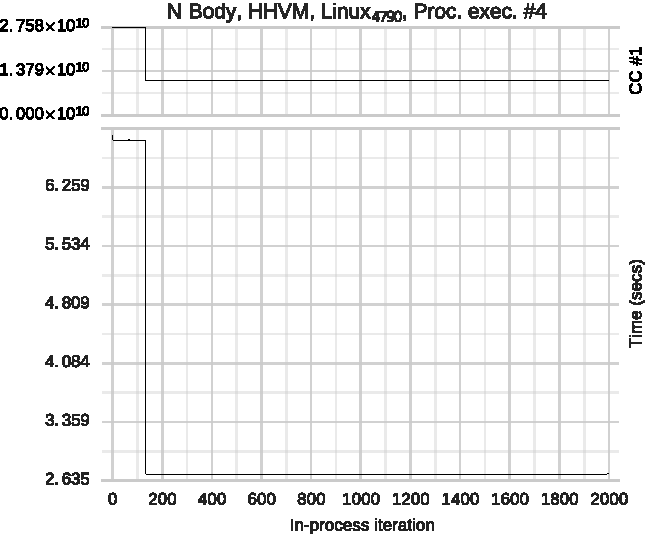
\includegraphics[width=.45\textwidth]{examples/new_warmup_no_migrate.pdf}
\caption{An example of traditional warmup behaviour with the n-body benchmark on
HHVM (process execution 4 of 10 run on \bencherthree). The run-sequence plot
(bottom) shows that warmup completed by in-process iteration \#134. The
core-cycle plot (top) shows that the main benchmark computation
occurred almost entirely on core 1: cores 0, 2 and 3 had Cycle Counts (CC) close
to 0 for the entire in-process execution and are thus elided.}
\label{fig:examples:trad}
\end{figure}

\begin{figure}[t]
\centering
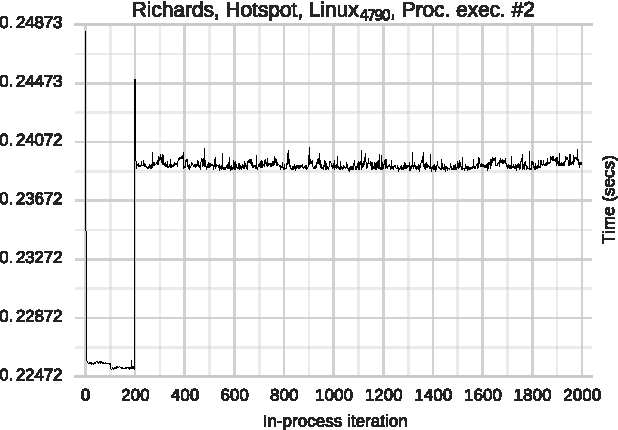
\includegraphics[width=.45\textwidth]{examples/new_slowdown.pdf}
\caption{Slowdown at in-process iteration \#199.}
\label{fig:examples:slowdown1}
\end{figure}

\begin{figure}[t]
\centering
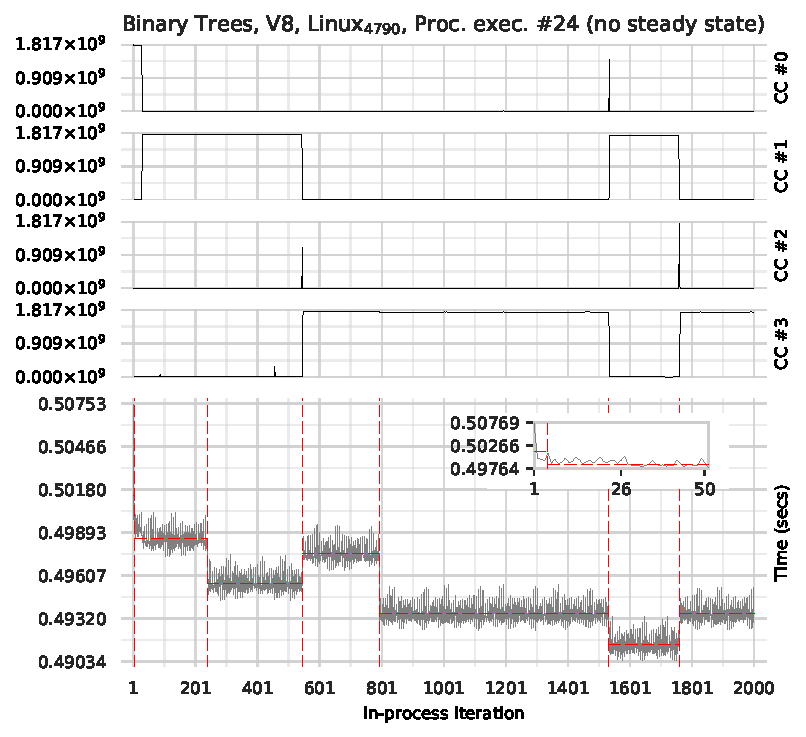
\includegraphics[width=.45\textwidth]{examples/new_no_steady.pdf}
\caption{No steady state. There is a small behavioural shift around iteration
950, where the VM migrates from (tickless) core 1 to (ticked) core 0.}
\label{fig:examples:nosteadystate}
\end{figure}

\begin{figure*}[t!]
\centering
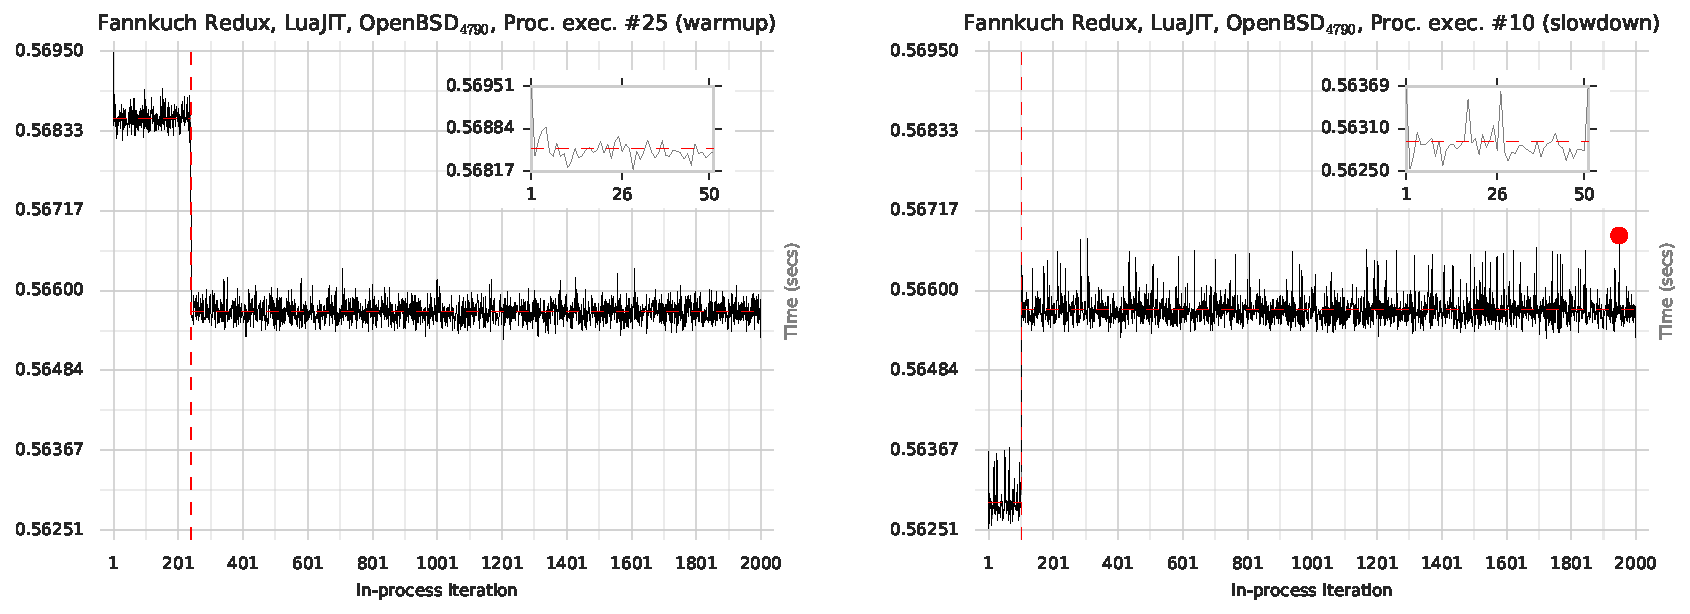
\includegraphics[width=\textwidth]{examples/new_inconsistent.pdf}
\caption{Examples of inconsistent process executions on the same system.}
\label{fig:examples:inconsistent}
\end{figure*}

Core-cycle plots help us understand how VMs use, and how the OS schedules,
threads. Benchmarks running on single-threaded VMs are characterised by a high
cycle-count on one core, and very low (though never quite zero) values on all
other cores. Such VMs may still be migrated between cores during process
execution, as can be clearly seen in Figure~\ref{fig:examples:nosteadystate}.
Multi-threaded VMs can run JIT compilation and / or GC in parallel:
Figure~\laurie{XXX maybe show the core cycle counts for hotspot/richards?} shows
an example. It is often hard to detect parallelism in the resulting core counts as
the main benchmark computation tends to be frequently migrated between cores:
however, it can often easily be seen that several cores are active during the first few
in-process iterations whilst JIT compilation occurs.

The APERF/MPERF ratio plots (see the Appendix for
examples) allow us to see if the processor's frequency changed during
benchmarking. The error in reading these values is relatively high (see
Section~\ref{aperf/mperf error}). Thus whilst in an ideal world we would
insist that the APERF/MPERF ratio should always be exactly 1, we have to apply a
small amount of discretion. We wrote a simple automated analysis that checks the
APERF/MPERF data; any core whose cycle count for a given in-process iteration is
below \laurie{XXX} is ignored; `active' cores are then checked for an
APERF/MPERF ratio between \laurie{i guess something like 0.97 and 1.03?}.


\subsection{Cyclic data}

\begin{figure}[tbp]
\centering
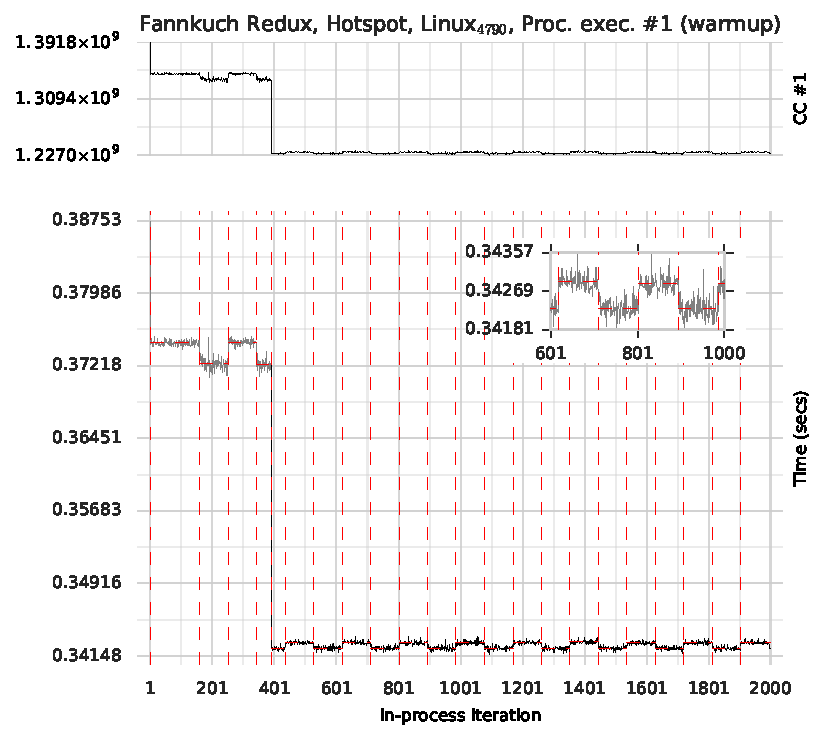
\includegraphics[width=.45\textwidth]{examples/new_cyclic.pdf}
\caption{Cycles in wall-clock times and core-cycle counts.}
\label{fig:examples:cycles}
\end{figure}

We suspected that enough benchmarks
would exhibit cyclic behaviour (as seen in Figure~\ref{fig:examples:cycles}) to
require special support in our automated analysis; and a by-eye glance at
data seemed to confirm this. In order to gain a more rigorous
understanding, we took one process
execution from each benchmark run on \bencherthree, removed the first 1500
in-process iterations, and plotted an autocorrelation graph for the remainder
(in similar fashion to \kalibera). Only 4 benchmarks showed what we have come to
call `fully cyclic' behaviour, where all in-process iterations repeat in a
predictable pattern. A further 8 showed `partially cyclic' behaviour, where
most iterations are noise around a mean, but every $n$ iterations there is a
predictable and significant peak in-process iteration (with $n$ varying from 5
to 19).

For partially cyclic data, or fully cyclic data with a large cycle-length (as in
Figure~\ref{fig:examples:cycles}), our automated analysis handles the situation
appropriately (in the specific example, classifying it as no steady state).
However, identifying small cycle lengths in fully cyclic data is
an open research challenge in changepoint analysis. Since it is so rare (only 2
of our benchmarks, in both cases with a small absolute difference between the
elements of the cycle), we do not consider this a significant problem in practice.


\subsection{The Effects of Compilation and GC}
\label{sec:deepdive}

The large number of non-warmup cases in our data led us to make the following hypothesis:
\begin{description}
  \item[H3] Non-warmup process executions are largely due to JIT compilation or GC.
\end{description}
To test this hypothesis, we made use of the that both HotSpot and PyPy allow
information about the duration of JIT compilation and GC to be recorded. Since
recording this additional data could potentially change the results we collect,
it is only collected when \krun is explicitly set to `instrumentation mode'. An
example instrumentation-plot can be seen in Figure~\laurie{XXX}.

\laurie{discuss the effect once we've got the data}


\section{Startup Time}
\label{sec:startup}

The data presented thus far in the paper has all been collected after the VM has
started executing the user program. The period between a VM being initially
invoked and it executing the first line of the user program is the VM's \emph{startup} time,
and is an important component in understanding a VM's real-world performance.

A small modification to \krun enables us to measure startup. We prepend each VM
execution command with a small C wrapper, which prints out wall-clock time
before immediately executing the VM itself; and, for each language under
investigation, we provide a `dummy' iterations runner which simply prints out
wall-clock time. In other words, we measure the time just before the VM is loaded
and at the first point that a user-level program can execute code on the VM; the
delta between the two is the startup time. For each VM we run 200 process
executions (note that, for this measure, in-process executions are irrelevant,
as the user-level program completes as soon as it has printed out wall-clock
time). Figure~\laurie{XXX} shows the data for each of our
3 benchmarking machines. As this data clearly shows, there is substantial
variation in the startup time of various VMs.


\section{Applying the Statistical Method to Existing Benchmark Suites}
\label{sec:existing}

\begin{table}[t]
\centering
\input{dacapo.table}
\caption{Dacapo results.}
\label{tab:dacapo}
\end{table}

The statistical method presented in Section~\ref{sec:stats} is not limited to data
produced from Krun. To demonstrate this, we have applied it to two standard
benchmark suites: DaCapo~\cite{dacapo06} (Java) and Octane~\cite{octane}
(JavaScript). We ran both for 10 process executions and 2000 in-process
iterations without reboots, temperature control etc.: DaCapo on \bencherthree;
and Octane on \bencherseven (a Xeon machine, with a software setup
identical to \bencherthree).\footnote{The large amount of CPU time our
experiments require meant that we ran out of time to run Octane on \bencherthree
before paper submission. For the final paper, we will run DaCapo and Octane on
the same machine. Although we do not expect this to result in significant
changes to the data, it will reduce a source of variation.}

We ran DaCapo (with its default benchmark size) on Graal and HotSpot. As it already has support for
altering the number of in-process executions, we used it without modification.
However, we were unable to run 4 of its 14 benchmarks: \texttt{batik}
crashes with a \texttt{Invocation\-Target\-Exception}; \texttt{eclipse},
\texttt{tomcat}, and (intermittently) \texttt{tradesoap} fail their own internal
validation checks.

We ran Octane on SpiderMonkey (\#465d150b, a JIT compiling VM for JavaScript) and V8.
We replaced its complex runner (which reported timings with a non-monotonic
microsecond timer) with a simpler alternative (using a monotonic millisecond
timer). We also had to decide on an acceptable notion of `iteration'. Many of Octane's
benchmarks consist of a relatively quick `inner benchmark'; an `outer benchmark'
specifies how many times the inner benchmark should be run in order to make an
adequately long running benchmark (very roughly, around 1s on \bencherseven, for
example). We recorded 2000 iterations of the outer benchmark; our runner
fully resets the benchmark and the random number generator between each
iteration. The \texttt{box2d}, \texttt{gameboy}, \texttt{mandreel} benchmarks do
not properly reset their state between runs, leading to run-time errors we have
not been able to fix; \texttt{typescript}'s reset function, in contrast, is
overzealous, freeing constant data needed by all iterations, which we were able
to easily fix. When run for 2000 iterations, \texttt{CodeLoadClosure},
\texttt{pdfjs}, and \texttt{zlib} all fail due to memory leaks. We were able to
easily fix \texttt{pdfjs} by emptying a global list after each iteration,
(a patch has been submitted to, but not yet accepted, to Octane), but not the
others. We therefore include 12 of Octane's benchmarks (including lightly
modified versions of \texttt{pdfjs} and \texttt{typescript}).
Because we run fewer benchmarks, our modified runner is unable to fully
replicate the running order of Octane's original runner. Since Octane runs all
benchmarks in a single process execution, this could affect the performance of
later benchmarks in the suite.

Table~\ref{tab:dacapo} shows the DaCapo results and Table~\ref{tab:octane} (in
the Appendix) the Octane results.


\section{Threats to Validity}
\label{sec:threats}

While we have designed our experiment as carefully as possible, we do not
pretend to have controlled every possibly confounding variable. Indeed, our
designing the experiment has been one of continually uncovering
confounding variables whose existence we had not previously imagined. It
is inevitable that there are further confounding variables that we
do not know about; some of these may be controllable, although many may not be.
It is possible that confounding variables that we are not aware of have
coloured our results.

We have tried to gain a partial understanding of the effects of different
hardware on benchmarks by using machines with the same OS but
different hardware. However, while the hardware between the two is
different, much more distinct hardware (e.g.~a non-x86 architecture) is
available, and is more likely to uncover hardware-related differences.
However, hardware cannot be varied in isolation from software:
the greater the differences in hardware, the more likely that JIT compilers
compilers are to use different code paths (e.g.~different code generators and
the like). Put another way, an apples-to-apples comparison across very different
hardware is likely to be impossible, because the `same' software in fact has
different behaviour on the different platforms.

We have not systematically tested whether rebuilding VMs effects warmup, an
effect noted by \kalibera, though which seems to have little effect on
the performance of JIT compiled code~\cite{barrett15approaches}. However, since measuring warm-up largely
involves measuring code that was not created by a JIT compiler, it is possible
that these effects may impact upon our experiment. To a limited extent, the
rebuilding of VMs that occurred on each of our benchmarking machines gives
some small evidence as to this effect, or lack thereof.

The checksums we added to benchmarks ensure that, at a user-visible level, each
performs equivalent work in each language variant. However, it is impossible to
say whether each performs equivalent work at the lowest level or not. For
example, choosing to use a different data type in a language's core library may
substantially impact performance. There is also the perennial problem as to the
degree to which an implementation of a benchmark should respect other
language's implementations or be idiomatic (the latter being likely to
run faster). From our perspective, this possibility is somewhat less important,
since we are more interested in the warmup patterns of reasonable programs,
whether they be the fastest possible or not. It is however possible that by
inserting checksums we have created unrepresentative benchmarks, though
this complaint could arguably be directed at the unmodified benchmarks too.

\laurie{with luck, the APERF/MPERF ratios will allow us to shorten this paragraph
and say ``our data shows this did not affect our experiment''. We'll see!} Although \krun does as much to control CPU clock speed as possible, modern CPUs
do not always respect operating system requests. Even on Linux, where we control
the CPU's P-state, we cannot guarantee that this fixes the CPU frequency: as
the Linux kernel documentation states, ``the idea that frequency can be set to a single
frequency is fiction for Intel Core processors''~\cite{pstate}. In
some cases, changes the CPU makes to its performance are detected and reported
by the operating system (e.g.~performance throttling due to potential
overheating); in other cases, changes may go undetected or unreported.
Despite this, our benchmarks show fairly predictable performance across
different hardware, suggesting that the effect of CPU performance changes may
not be significant in our case.

Although we have minimised the number of system calls that our in-process
iterations runners make, we cannot escape them entirely. For example,
on both Linux and OpenBSD, \texttt{clock\_gettime()} (which we use to obtain
monotonic wall-clock time) contains what is effectively a spin-lock,
meaning that there is no guarantee that it returns within a fixed bound.
%\footnote{See \texttt{binuptime} in \texttt{sys/kern/kern\_tc.c} in the
%OpenBSD source code and \texttt{getrawmonotonic} in
%\texttt{kernel/time/timekeeping.c} in the Linux source code.}
In practise, \texttt{clock\_gettime} returns far quicker than the granularity
of any our benchmarks, so this is a minor worry at most. \label{aperf/mperf error} The situation
on Linux is complicated by our reading of core cycle and APERF/MPERF
counts via MSR device nodes: we call \texttt{lseek} and \texttt{read}
between each in-process iteration (we keep the files open across all
in-process iterations to reduce the open/close overhead).
These calls are more involved than \texttt{clock\_gettime} \laurie{let's put a
figure on it}. As well as the filesystem overhead, reading from a MSR device
node triggers inter-processor interrupts to schedule an \texttt{RDMSR}
instruction on the desired core (causing the running core to save its registers etc.). We
were not able to find a lighter-weight timing mechanism, despite trying
candidates such as the x86 Time Stamp Counter (TSC). On older systems the TSC
increments relative to the CPU's frequency (and thus can be indirectly used to
detect CPU frequency changes); on modern systems, its readings are always
normalised to a fixed CPU frequency (and its readings are thus immune from CPU
frequency changes).

Our experiments allow the kernel to run on the same core as benchmarking code.
We experimented extensively with CPU pinning, but eventually abandoned it. After
being confused by the behaviour of Linux's \texttt{isolcpus} mechanism (whose
semantics changes between a normal and a real-time kernel), we used CPU shielding
(\texttt{cset shield}) to pin the benchmarks to the 3 non-boot cores on our
machines. However, we then observed notably worse performance for VMs such as
HotSpot. We suspect this is because such VMs query the OS for the number of
available cores and create a matching number of compilation threads; by reducing
the number of available cores, we accidentally forced two of these threads to
compete for a single core's resources.

In controlling confounding variables, our benchmarking environment necessarily
deviates from standard configurations. It is possible that in so doing, we have
created a system that shows warmup effects that few people will ever see in
practise. However, our judgement is that this is preferable to running on a
noisy system that is likely to introduce substantial noise into our readings.


\section{Related work}

There are two works we are aware of which explicitly note unusual warmup
patterns. Whilst running benchmarks on HotSpot, Gil et
al.~\cite{gil11microbenchmark} experienced inconsistent process executions
(e.g.~recursiveErgodic), and benchmarks that we could classify as no
steady state (listBubbleSort) and slowdown (arrayBubbleSort). By running a
larger number of (somewhat larger) benchmarks on a number of VMs, and executing
them in a more tightly controlled execution environment, our results can be seen
as significantly strengthening Gil et al.'s observations. Our work also adds an
automated approach to identifying when warmup has occurred.
\kalibera note the
existence of what we have called cyclic behaviour (in the context of benchmarking,
they then require the user to
manually pick one part of the cycle for measurement~\cite{kalibera13rigorous}):
the data from our experiment seems to be less often cyclic, though we have no
explanation for why.


\section{Conclusions}
\label{sec:conclusion}

Warmup has previously been an informally defined term~\cite{seaton15phd} and in this
paper we have shown cases where the definition fails to hold. Through a carefully
designed experiment, and an application of a new statistical method, we hope
to have helped give the study of warmup a firmer base.

Although we are fairly experienced in designing and implementing
experiments, the experiment in this paper took far more time than we expected
--- about 2 full person years. In part this is because there is limited precedent for such detailed
experiments. Investigating possible confounding variables, understanding how to
control them, and implementing the necessary checks, all took time. In many
cases, we had to implement small programs or systems to understand a variable's
effect (e.g.~that Linux allows a process to allocate memory beyond that
specified in the soft and hard \texttt{ulimit}). However, we are realistic that
few people will have the time or energy to institute all the controls that we
implemented. An open question is which of the controls are the most significant
in terms of producing a reliable experiment. The large number of partly
inter-locking combinations means that we estimate that untangling this will
require 3--6 months of experimental running time.

Our results have suggested to us some potentially useful advice for VM
developers and users. First, simply running benchmarks for a larger number of
in-process iterations is a simple way of understanding a VM's long-term
performance stability. Second, as a community, we need to accept that a steady
state of peak performance is not guaranteed to exist. Third, the significant
differences in warmup time between VMs strongly suggest that VM benchmarking
should always include warmup time. Fourth, we suspect that some of the odd
results we have seen result from over-training VM heuristics on small sets of
benchmarks. The approach taken by the machine-learning community may be apply
equally well to the VMs: using a training set to devise heuristics, and then
benchmarking the resulting system(s) on a separate validation system. Fifth, we suspect
that the general reliance on small suites of benchmarks means that only
small parts of VMs are being benchmarked effectively: we are increasingly of the
opinion that benchmarking quality and quantity are tightly related, and that VMs
need more benchmarks.

\textbf{Transparency:} Three of this paper's authors have contributed
substantial code to the PyPy project. The King's group has received
several funding gifts from Oracle Labs.

\textbf{Acknowledgements:} We are particularly grateful to Vincent Knight
who helped put together the team that made this paper. We also thank (in alphabetical order) Dave Dice, Kenny
Gross, Tim Harris, Dave Ungar, Mario Wolczko for comments and suggestions; any
errors and infelicities are our own. This research was funded by the EPSRC
Cooler (EP/K01790X/1) grant and Lecture (EP/L02344X/1) fellowship.

\bibliographystyle{plain}
\bibliography{bib}

\newpage

\appendix

\section{Main Results}
\label{app:mainresults}

\laurie{the results for the other 2 benchers should go here}


\section{Octane Results}

\begin{table}[t]
\centering
\input{octane.table}
\caption{Octane results.}
\label{tab:octane}
\end{table}

\end{document}

